\begin{figure}[!h]
  \centering
  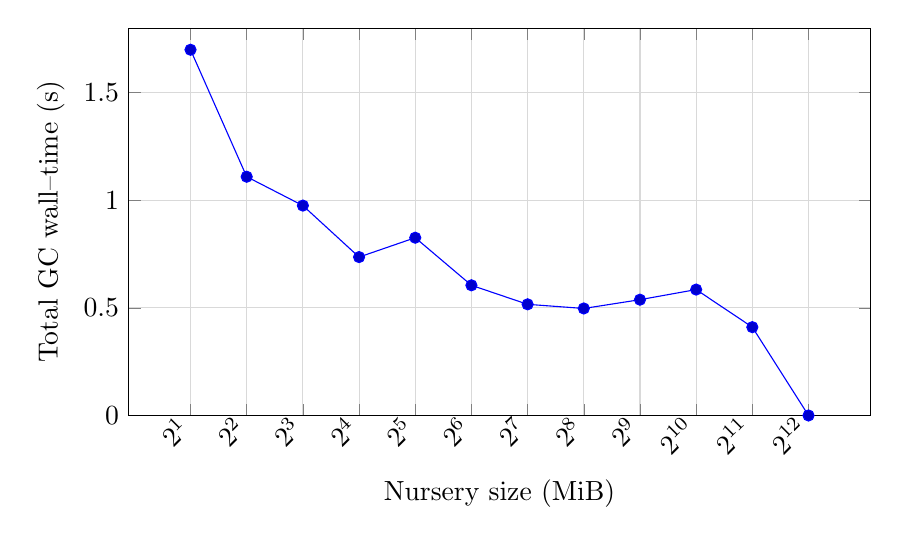
\begin{tikzpicture}
    \begin{axis}[
      width=11cm,
      height=6.5cm,
      xmode=log,
      log basis x=2,
      xlabel={Nursery size (MiB)},
      ylabel={Total GC wall--time (s)},
      ymin=0,
      ymax=1.8,
      xtick={2,4,8,16,32,64,128,256,512,1024,2048,4096},
      xticklabel style={rotate=45, anchor=east},
      grid=major,
      mark options={solid},
      every major grid/.style={gray!30},
    ]
      \addplot+[mark=*] coordinates {
        (2,     1.69996)
        (4,     1.10974)
        (8,     0.975673)
        (16,    0.736303)
        (32,    0.826354)
        (64,    0.605177)
        (128,   0.516714)
        (256,   0.497457)
        (512,   0.538291)
        (1024,  0.585262)
        (2048,  0.41057)
        (4096,  0.000048)
      };
    \end{axis}
  \end{tikzpicture}
  \caption{Effect of nursery size on total GC wall--time for Pycket with self-hosting.}
  \label{figure:nursery-size-vs-gc-time}
\end{figure}
